% 五号字体,开明式标点处理,不设置默认字体
\documentclass[UTF8,12pt,punct=kaiming,fontset=none]{ctexart}
\usepackage{fontspec}  % 字体
\usepackage{subcaption}  % 节标题
% 链接和注释
\usepackage[pageanchor,colorlinks=true,linkcolor=black,citecolor=black,urlcolor=black,linktoc=none]{hyperref}
\usepackage{geometry}  % 页面布局
\usepackage{fancyhdr}  % 页眉页脚
\usepackage{titlesec}  % 标题
\usepackage{graphicx}  % 图片路径
\usepackage[pages=some]{background}  % 封面
\usepackage{bookmark}  % 书签
\usepackage{anyfontsize}  % 字体大小
\usepackage{ifthen}  % 判断
\usepackage{wrapfig}  % 文字并排图片
\usepackage{setspace} % 行距

% 图片路径
\graphicspath{{figures/}}

% 封面
% \backgroundsetup{
%     scale=1,
%     color=black,
%     opacity=1,
%     angle=0,
%     contents={
%         \includegraphics[width=\paperwidth,height=\paperheight]{封面.png}
%     }
% }

% 字体
\setCJKmainfont{Source Han Serif SC}
\setCJKsansfont{Source Han Sans SC}
\setmainfont{CMU Serif}

% 布局
\geometry{a4paper,left=2cm,right=2cm,top=2.5cm,bottom=2.5cm}
\setlength{\headheight}{25pt}

% 页眉页脚
\pagenumbering{arabic}
\pagestyle{fancy}
\fancyhead[L]{· \hspace{0.1cm} \thepage \hspace{0.1cm} ·}
\fancyhead[C]{红 \hspace{0.08cm} 石 \hspace{0.08cm} 数 \hspace{0.08cm} 电 \hspace{0.08cm} 评 \hspace{0.08cm} 论\\\scriptsize{Review of Redstonic Digital Circuit}}
\fancyhead[R]{第1期\\\scriptsize{2022年2月}}
\fancyfoot[L,C,R]{}

% 首页页码
\setcounter{page}{1}

% 无首行缩进
\setlength\parindent{0pt}

\begin{document}

% 封面
\thispagestyle{empty}
\BgThispage
\quad
\newpage

% 标题
\quad
\vspace{-0.3cm}
\begin{center}
    \fontsize{46pt}{54.2pt} \textbf{红石数电评论} \\
    \Large Review of Redstonic Digital Circuit \\
    \Large 第1期(2022年2月)
\end{center}

% 目录
\makeatletter
\newcommand{\cdotfill}{\leavevmode\cleaders\hb@xt@ 0.56cm{\hss\ensuremath{\cdots}\hss }\hfill\kern\z@}
\makeatother
\newcounter{currentPageNumber}
\setcounter{currentPageNumber}{3}
\newcounter{nextPageNumber}
\newcommand{\addContent}{
    \setcounter{nextPageNumber}{\arabic{currentPageNumber}}
    \ifthenelse{\pageNumber>1}{
        \addtocounter{nextPageNumber}{\pageNumber}
        \addtocounter{nextPageNumber}{-1}
        \hyperlink{page.\arabic{currentPageNumber}}{\fileName\cdotfill\authorName\quad\arabic{currentPageNumber} - \arabic{nextPageNumber}}
    }{
        \hyperlink{page.\arabic{currentPageNumber}}{\fileName\cdotfill\authorName\quad\arabic{currentPageNumber}}
    }
    \bookmark[page={\arabic{currentPageNumber}}]{\fileName}
    \addtocounter{currentPageNumber}{\pageNumber}
    
}

% TODO: 自动填写模板

\begin{spacing}{2.0}

% 论文
% \addtocontents{toc}{\string\contentsline{part}{论文}{}{}}
\large\sffamily\bfseries 论文

\normalsize\normalfont
\input{论文.inc}

% 通讯
% \addtocontents{toc}{\string\contentsline{part}{通讯}{}{}}
\large\sffamily\bfseries 通讯

\normalsize\normalfont
\input{通讯.inc}

\end{spacing}

\vspace{1cm}

% 版权页
\begin{spacing}{1.5}
\begin{wrapfigure}{r}{0.25\linewidth}
    \vspace{-2.5cm}
    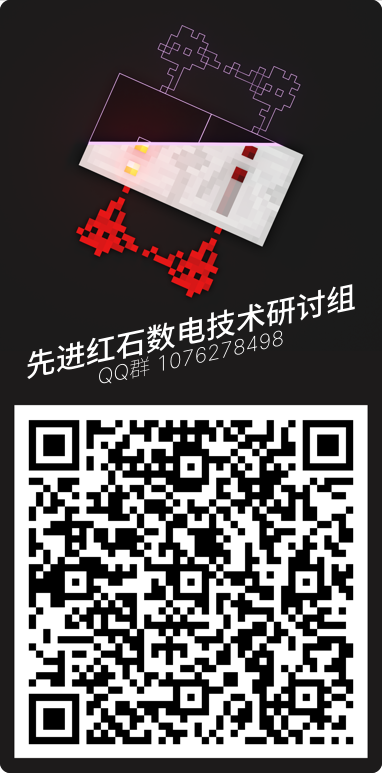
\includegraphics[width=\linewidth]{qrcode.png}
\end{wrapfigure}    
\hspace{1cm}
\begin{minipage}[c]{0.55\linewidth}
    \titleformat{\section}[leftmargin]{\sffamily\bfseries}{}{0cm}{}
    \titlespacing{\section}{1.2cm}{1ex}{0cm}

    \section*{主办}
    先进红石数电技术研讨组(ARS)

    \section*{编辑}
    @辰占鳌头\hspace{0.5cm}@NKID00

    \section*{封面}
    @NKID00

    \section*{链接}
    \url{https://github.com/ARS-MC/RRDC}

    \section*{投稿}
    \href{https://github.com/ARS-MC/RRDC/issues/new?assignees=&labels=%E6%8A%95%E7%A8%BF&template=contribute.md&title=%E5%9C%A8%E6%AD%A4%E5%A4%84%E5%A1%AB%E5%86%99%E6%A0%87%E9%A2%98}{在GitHub存储库中提交issue} 或扫描右侧 QR 码加入 QQ 群
\end{minipage}
\end{spacing}

\end{document}
